\let\mypdfximage\pdfximage
\def\pdfximage{\immediate\mypdfximage}
\documentclass[11pt]{article}

\usepackage{bridges}
\usepackage{rotating} %% For the sideways
\usepackage{graphicx} %% For including pretty pictures
\usepackage{url}      %% For formatting URLs.
\usepackage{amsmath}  %% for \text
\usepackage{amssymb}  %% for the square

\title{\textbf{People and Computers Agree on the Complexity of Small Art}}

\author{
	Peter Boothe \\
	Google, New York, NY \\
	Manhattan College, Riverdale, NY \\
	\url{pboothe@gmail.com} \\
	\\
	Jonathan Langke \\
	Manhattan College, Riverdale, NY \\
	\url{jlangke22@gmail.com}
}

\date{}

\bibliographystyle{plain}

%% Set the indentation at the start of paragraphs.
\setlength{\parindent}{0.3in}

%% Set the spacing between paragraphs.  The guidelines don't specify
%% that there should be a space, but I find paragraphs hard to read
%% without it.  I'm inserting a small space that you may choose to
%% modify.
\setlength{\parskip}{.65ex}

\begin{document}
\maketitle

%% Make sure not to include a page number on the first page.
\thispagestyle{empty}

\begin{abstract}

Restricting our purview to black and white digital artworks on a grid, we
developed a lower-power version of Kolmogorov complexity, and then we found the
complexity of every piece of 3x3 art.  We also asked people to compare two
artworks and decide which one was more visually complex as they understood the
term.  We used these comparisons to assign every artwork a strength rating
(similar to a chess rating), and we found that the human-generated ratings were
well correlated with the formula complexity of the artworks.  Therefore,
computers and humans largely agree on the complexity of small artworks!

\end{abstract}

\section*{Introduction}

We compare the complexity of small artworks from two perspectives: that of a
computer, and that of a human.  To do this in a principled manner we define our
artworks, define our notion of complexity for computers, and describe how we
measured visual complexity for people.  We proceed through each task in turn,
one per section, before bringing our computer and human results
together and describing future work in the last sections.

\section*{Our Definition of Art \& Artworks}

In order to make this question tractable, and in order to ensure that our
artworks are ``native'' to both the human and computer domains, we restrict our
purview to black and white pixel-based digital artworks.  This is clearly a
subset of all digital artworks, but it is still an expressive subset, as shown
in Figure~\ref{fig:monalisa}.  

We can generate a mapping of positions on the grid to black and white pixels in
multiple ways.  The simplest way to generate the mapping is to simply write
down the sequence verbatim: white, black, black, white, etcetera.  However,
considered more generally, each artwork can also be thought of as the output of
a function that takes two numbers as input (representing the grid position of
each pixel) and returns either true or false (representing whether the pixel at
that position is black or white).  In computer science terms, every black and
white picture is the output of a function of type {\tt
int$\times$int$\to$bool}.  

\begin{figure} 
\begin{center} 
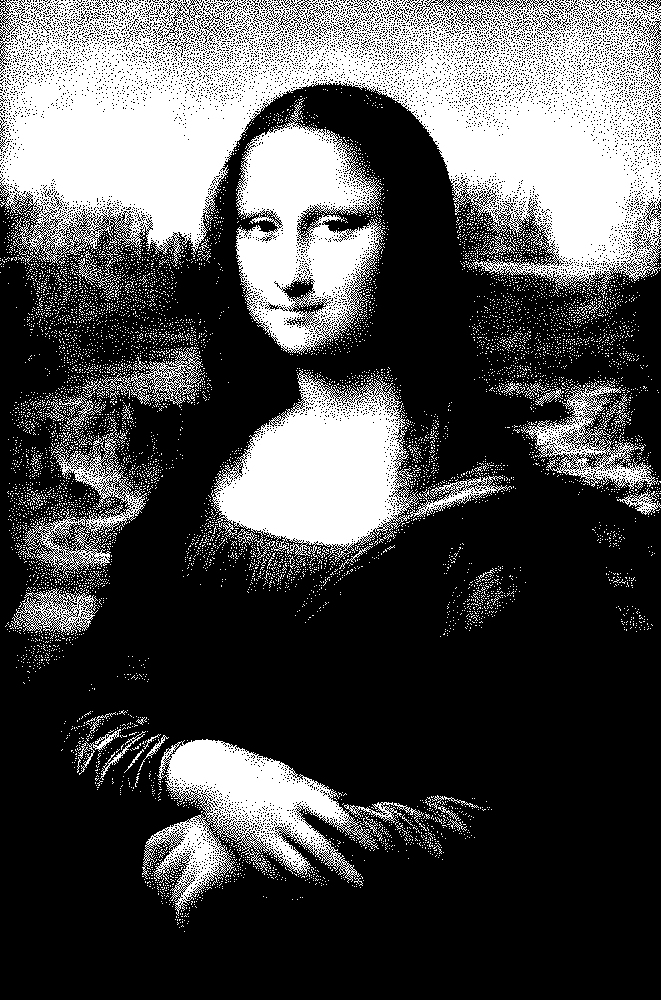
\includegraphics[width=5in]{monalisa_mono.jpg}
\end{center} 
\caption{This version of the Mona Lisa consists solely of black
and white (and no gray) pixels on a grid, and can therefore be considered
either as a picture, or as the output of a function of type {\tt
int$\times$int$\to$bool} that maps integer grid positions to black and white
truth values.  This image has more pixels than any artwork we consider, but
serves as an effective argument that art can result from the evaluation of a
function of type {\tt int$\times$int$\to$bool}.}
\label{fig:monalisa} 
\end{figure}

This isomorphism between the output of functions of type {\tt
int$\times$int$\to$bool} and black and white artworks is the basis of our work,
as it allows us to ask people about the perceived visual complexity of an
artwork, and to ``ask'' computers about the complexity of the corresponding
functions.  In order to make our problems computationally tractable, we
restrict our purview to artworks that are nine pixels laid out in a three by
three grid.  This allows us to generate all artworks (of which there are
$2^9=512$), and also, less trivially, to enumerate all possible formulae in an
effort to calculate the formula complexity of each artwork.

\begin{figure}
\begin{tabular}{c r r}
3x3 Artwork & Formula Complexity & Formula of minimum size \\
\hline
\reflectbox{\rotatebox[origin=c]{180}{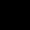
\includegraphics[width=.75in]{3x3pics/0.png}}} & 1 & {\tt true } \\
\reflectbox{\rotatebox[origin=c]{180}{
\includegraphics[width=.75in]{3x3pics/500.png}}} & 5 & {\tt (1 < (x + y))} \\
\reflectbox{\rotatebox[origin=c]{180}{
\includegraphics[width=.75in]{3x3pics/122.png}}} & 16 & {\tt ((not (x < (x * y))) and ((x * x) < (x + (x + y))))}

\end{tabular}
\caption{Some example artworks, listed with their formula complexity and a formula with that complexity.  Black corresponds to true and gray to false, and the bottom left corner is pixel $(0,0)$.}
\label{fig:artexamples}
\end{figure}

\section*{Formula Complexity}

Formula complexity is intended to be a ``low power'' version of Kolmogorov
complexity\footnote{This complexity measure was independently invented at least
three times, by Chaitin, Solomonoff, and Kolmogorov.  The standard text is Li
and Vit\'anyi~\cite{Li}, although Chaitin's article in Scientific
American~\cite{chaitin} and Aaronson's article in American
Scientist~\cite{aaronson} both provide very readable introductions.}.  In
Kolmogorov complexity, the complexity of an object is defined to be the size of
the smallest program that outputs that object --- interestingly, the
programming language used does not usually matter, as all Turing-complete
programming languages are equivalent up to an additive constant.

Kolmogorov complexity is uncomputable, and so has largely been ignored when
people engage in practical computation regarding specific objects.  Frequently,
researchers use compression programs to find out how much a file can be
compressed, and they consider that compressed size to be an approximation of
the Kolmogorov complexity.  Unfortunately, using a compression program results
in an estimate that can be off by an arbitrary amount.  Kolmogorov complexity
is not just uncomputable to calculate, it is uncomputable to approximate!  In
our effort to be exact, we turn to an alternative measure.

Formula complexity is also a property of an object, in this case a
2-dimensional artwork, but the programming language used to write the function
of type {\tt int$\times$int$\to$bool} is not Turing-complete.  In particular,
in formula complexity it is impossible to define and call functions, which
prohibits looping and recursion.  Instead of the entirety of mathematical
symbols, in formula complexity we restrict ourselves to just the symbols in the
set $\{\text{\tt +, *, 0, 1, x, y, true, false, not, and, or, <}\}$. To
eliminate any potential ambiguity of interpretation we require that every
expression be fully parenthesized.  The symbols {\tt x} and {\tt y} in each formula
represent the coordinates of the grid point being interpreted.  

The set of symbols in our language was selected based on its mathematical
minimalism and the completeness of each operation.  For example, 0, 1, and
multiplication and addition were included because they collectively ensure that
any number $n$ can be represented using at most $O(\log^2 n)$ symbols instead
of the $2n-1$ symbols that including only 1 and addition would require.  Division
was not included because division is not defined on all inputs, which means
that we would have to worry about formulae with undefined values.  The
less-than operation was included as a method of converting integers to boolean
values, but the greater-than operation was not included because it is
equivalent to the less-than operation with the operands reversed.  Mathematical
minimalism of the symbol set is important for practical reasons due to the
exponential explosion of the number of formulae of size $n$. 

If we consider only the binary operations (temporarily neglecting the {\tt not}
operation), then the number of formulae of size $n$ is equal to the product of:
the number of full binary trees with $n$ nodes (the $n-1$ Catalan number); the
number of assignments for the $\lfloor n/2 \rfloor$ internal nodes (the number
of operations in our set raised to the $\lfloor n/2 \rfloor$ power); and the
number of assignments of values to the $\lceil n/2 \rceil$ leaf nodes (the
number of values in our set raised to the $\lceil n/2 \rceil$ power).
Therefore, for a given $n$, neglecting the complication of the {\tt not}
operation, the number of formulae is: 
\[C_{n-1} \cdot 5^{\lfloor n/2 \rfloor} \cdot 6^{\lceil n/2 \rceil}\]
This exponential growth means that as $n$ grows, the number of formulae of size
$n$ quickly becomes impractical for a computer.  This extreme growth, more than
anything else, is what forces us to keep our artworks small and our symbol set
minimal.

Note that some formulae that our symbol set can produce might make no sense.  For
example, the formula {\tt (1 + false)} requires adding a truth value to a
number.  Furthermore, other formulae produced may make sense, but not be useful
in our context because they do not evaluate to a truth value.  For example, if
our formula is {\tt (x + y)}, then what color should we make the pixel at
$(3,2)$?  Therefore, we place further restrictions on our formulae:
\begin{enumerate}
\item All formulae must be well-typed: numerical operations are only performed
on numbers (or subexpressions which evaluate to a number) and logical operations
are only performed on logical values (or subexpressions which evaluate to a
logical value).
\item All formulae must evaluate to {\tt true} or {\tt false} after
substituting the coordinate values in for {\tt x} and {\tt y}.
\end{enumerate}
The first requirement ensures that a formula makes sense, and the second
ensures that the formula can be used to define an artwork.  Now that these
preliminaries are decided, we can define formula complexity.

\begin{quote}\textbf{Definition (Formula Complexity)}~~The \emph{formula complexity} of an
artwork is the number of symbols used in the smallest formula which produces
that artwork when evaluated at each point on the grid.  
\end{quote}

We wrote a program to generate all well-typed formulae in order of size, and
then tested each formula as it was generated in order to determine if it was
the first formula to produce its corresponding 3x3 picture.  We ran our program for
months, but were only able to generate the formulae up to size 17 due to the
exponential explosion in formula count as formula size grows.  

Example artworks, along with their formula complexity and the corresponding
formula of minimum size, may be seen in Figure~\ref{fig:artexamples}.
Figure~\ref{fig:allthe3x3} contains a complete diagram of all artworks with
their corresponding formula complexity.

\begin{figure}
\begin{center}
\begin{sideways}
\input{3x3table.tex}
\end{sideways}
\end{center}

\caption{All the three by three artworks and the formula complexity of each.  The last category is labeled $\ge 17$ because the formula complexity of those artworks is unknown, except that it is at least 17.}
\label{fig:allthe3x3}
\end{figure}

\section*{Visual Complexity}

When compared with the mathematical formalism of formula complexity, visual
complexity is a frustratingly slippery concept.  We declined to define it at
all, instead allowing every survey participant to decide for themselves what it
meant.  We surveyed people online (through Twitter and through our own social
networks) and presented them with a page that showed two artworks and asked
them to click on the artwork that was more visually complex.  After they
clicked on one artwork, we presented them with another, and another, until
they decided for themselves to stop taking our survey.

To turn these pairwise comparisons into a rating of complexity,
we treated each survey response as a ``game result'' between the
two artworks. We turned the win-loss record of each artwork into a
strength rating using the TrueSkill algorithm~\cite{trueskill}, which is a
rating system similar to the one used in chess but with provably better
convergence times.

Just looking at the visual complexity data, we can find out whether our survey
participants ranked similar artworks as similarly complex.  Artworks can be
similar if one artwork is the negation of another (swapping black for white and
white for black), or if one artwork is the rotation or flip of another.  In
Figure~\ref{fig:differences}, we show the distribution of differences in visual
complexity rankings for randomly chosen artworks, and compare it to the visual
complexity rankings for artworks with a particular relation.

\begin{figure}
\begin{center}
\includegraphics[width=3.15in]{3x3onebit.pdf} 
\includegraphics[width=3.15in]{3x3swaps.pdf} 
\includegraphics[width=3.15in]{3x3inversions.pdf}
\end{center}

\caption{The differences between visual complexity rankings for related artworks, as compared with the differences between randomly selected artworks.  Artworks that differ by only one pixel or are flipped along the diagonal reliably have more similar strength rankings, while inverting the colors is more ambiguous.}
\label{fig:differences}
\end{figure}

In Figure~\ref{fig:differences}, we do some very basic investigation into our
visual complexity survey results.  In particular, we are looking to see if we
can characterize any differences that are important for people.  We do this by
engaging in pairwise comparisons between artworks that are different in a
particular way, and then comparing the distribution of visual complexity
differences of those pairs to the distribution of visual complexity distances
among all pairs.

When we look at artworks that only differ by a single pixel, we find that their
strength rankings are more likely to be similar than two randomly chosen
artworks.  The same is true for artworks that are the ``diagonal swap'' of one
another.  Interestingly, despite the computational triviality of swapping black
and white, it appears that the difference of visual complexity between artworks
that are the inverse of each other is not distinguishable from the difference
between two randomly chosen artworks.  Therefore, black and white were not
perceived as being interchangeable by our survey participants.

\section*{Comparing Complexity Results}

Armed with our computational results and our survey results, the only thing
left to do was see whether these two complexity rankings were well-correlated!
A complete chart of our results may be seen in Figure~\ref{fig:scatter}.  From
the figure, two things are clear: First, our correlation is definitely not
perfect because the dots do not form an increasing line; Second, there is some
correlation, because there are very few dots in the lower right or in the upper
left.

\begin{figure}
\begin{center}
\includegraphics[width=5in]{3x3scatter.pdf}
\end{center}
\caption{A scatter plot comparing visual complexity and formula complexity for
all 512 artworks, along with the line of best-fit.  The formula complexity is
artificially clamped at 17.  The correlation coefficient between the two
measurements is $.55$ and the p-value is $4\cdot10^{-39}$.} 
\label{fig:scatter}
\end{figure}

When we calculate Pearson's correlation coefficient, we get a correlation of
$.55$ and a very low p-value of $4\cdot10^{-39}$, which implies that it is safe
to reject the null hypothesis.  Therefore, we conclude that, for small digital
artworks, visual complexity is positively correlated with formula complexity!  

\section*{Conclusion and Future Work}

We defined a class of art that is explicable by both humans and computers.  We
also defined a ``powered down'' version of Kolmogorov complexity which we
called formula complexity and then calculated the formula complexity of all 3x3
artworks.  We asked people to compare artworks to each other and choose the one
that is most visually complex, and we assigned a complexity rating to each
artwork based on the number of comparisons it won and the strength of the
artworks it beat.  We then showed that these two, very different, complexity
measures are correlated.  From all this, we conclude that, for small digital
artworks, humans and computers agree about what is complex and what is simple!

The future work we lay out is related to the limits of both of our complexity
surveys, potential ways of increasing the power of our computer complexity
measure, and a search for a computer complexity measure that comes even closer
to the human one.

The computational survey was limited by available machine power.
It may be fruitful to run this computation again in a few years once transistor
density has increased.  Perhaps future programmers could find the formula
complexity of all of the small artworks.

Our human survey was limited to college students and Twitter friends.  Because
we are computer scientists, it is likely that the college students and
Twitter users we surveyed are not representative of the population at large.
Are we only seeing a correlation because we mostly surveyed people who had
taken CS classes? 

Other areas of math and CS have developed programming languages and formula
schema that allow for richer expressions. It might be interesting to try and
replicate this result using the simply-typed lambda calculus, which allows
function definition and just forbids recursion.  It may also be interesting to
try and replicate this result using Levin complexity, which is even closer to
Kolmogorov complexity.

Finally, and most interestingly, it could be quite fruitful to search for the
set of symbols which provide for a formula complexity that maximally matches the
measured visual complexity.  The discovery of this set of atoms would
potentially have deep implications for understanding how human brains perceive
the world!  All of our code and data is freely available online~\cite{Github} if
anyone would like to build upon it directly.

\bibliography{bibliography} 
\end{document}
